\chapter{技术基础}

\section{研究对象}

六个赛道覆盖三种基本学习问题。断层预测和地震相分割属于空间像素级预测；储层物性
预测、岩相分类和甜点评价属于表格或序列学习；三维重建属于稀疏观测条件下的空间
插值。不同任务共享同一研究目标：在不改变标签定义和数据划分的前提下，提高预测
精度，并说明增益来自何处。

\section{模型体系}

传统模型提供清晰而稳定的比较基准。逻辑回归用于像素二分类，FPN 和 DeepLabV3+
用于语义分割\cite{lin2017fpn,chen2018deeplabv3plus}，ExtraTrees、XGBoost、
CatBoost 和 LightGBM 用于表格预测\cite{geurts2006extratrees,chen2016xgboost,
prokhorenkova2018catboost,ke2017lightgbm}，普通克里金用于空间重建。基础模型则提供更丰富的预训练表征，包括 SAM-Med3D、
SAM2、TabICL、MOMENT、Chronos-2 和 OpenMind-MAE
\cite{wang2023sammed3d,ravi2024sam2,qu2025tabicl,goswami2024moment,
ansari2025chronos2,wald2025openmind}。

本项目不直接比较参数量，而是比较同一数据划分下的预测性能。若基础模型分支需要
融合，其输出只在开发集满足预设条件后进入最终预测。这样既保留传统模型在小样本
任务中的优势，也允许预训练模型在表征充分时发挥作用。

六个基础模型分支遵循同一归因逻辑。每个分支至少与赛道强基线比较；能够构造同结构
模型时，还要比较预训练初始化与随机初始化。融合模型必须单独评价无门控和受控融合，
并保持数据划分、输入信息与主要指标不变。该设计把研究问题从“是否使用大模型”
收敛为“预训练表征在何种数据条件下提供可重复的增量信息”。

\begin{table}[htbp]
  \centering
  \caption{六个赛道的任务、方法与主要实验结论}
  \label{tab:track-overview}
  \footnotesize
  \begin{tabularx}{\textwidth}{>{\raggedright\arraybackslash}p{2.05cm}YYY}
    \toprule
    赛道 & 输入与输出 & 主要方法 & 主要实验结论 \\
    \midrule
    断层预测 & 地震切片或体到断层概率 & 逻辑回归，SAM-Med3D & 二维基线可复现；三维评价数据不足 \\
    地震相分割 & 三通道切片到相类别图 & CNN，SAM2 交叉注意力 & 开发集 mIoU 提高，归因对照待补 \\
    储层物性预测 & 井曲线到 PHIF/KLOGH/SW & ExtraTrees，XGBoost，TabICL & 树模型留出结果稳定；TabICL 仅有初步开发证据 \\
    岩相分类 & 深度窗口到固定九类岩相 & XGBoost，MOMENT & MOMENT 优于随机初始化但弱于 XGBoost \\
    甜点评价 & 静态与生产信息到七项目标 & LightGBM，CatBoost，Chronos-2 & T3 开发集改善；其余目标分别评价 \\
    三维重建 & 稀疏井点到连续属性体 & 普通克里金，OpenMind-MAE 固定邻域核 & P21 在开发折与同场区历史版本上均降低 RMSE \\
    \bottomrule
  \end{tabularx}
\end{table}

\Cref{tab:track-overview}给出全文的比较主线。表中的“开发集改进”与“已知留出集
结果”具有不同证据强度，后续各章分别说明数据划分和适用范围。

\begin{figure}[htbp]
  \centering
  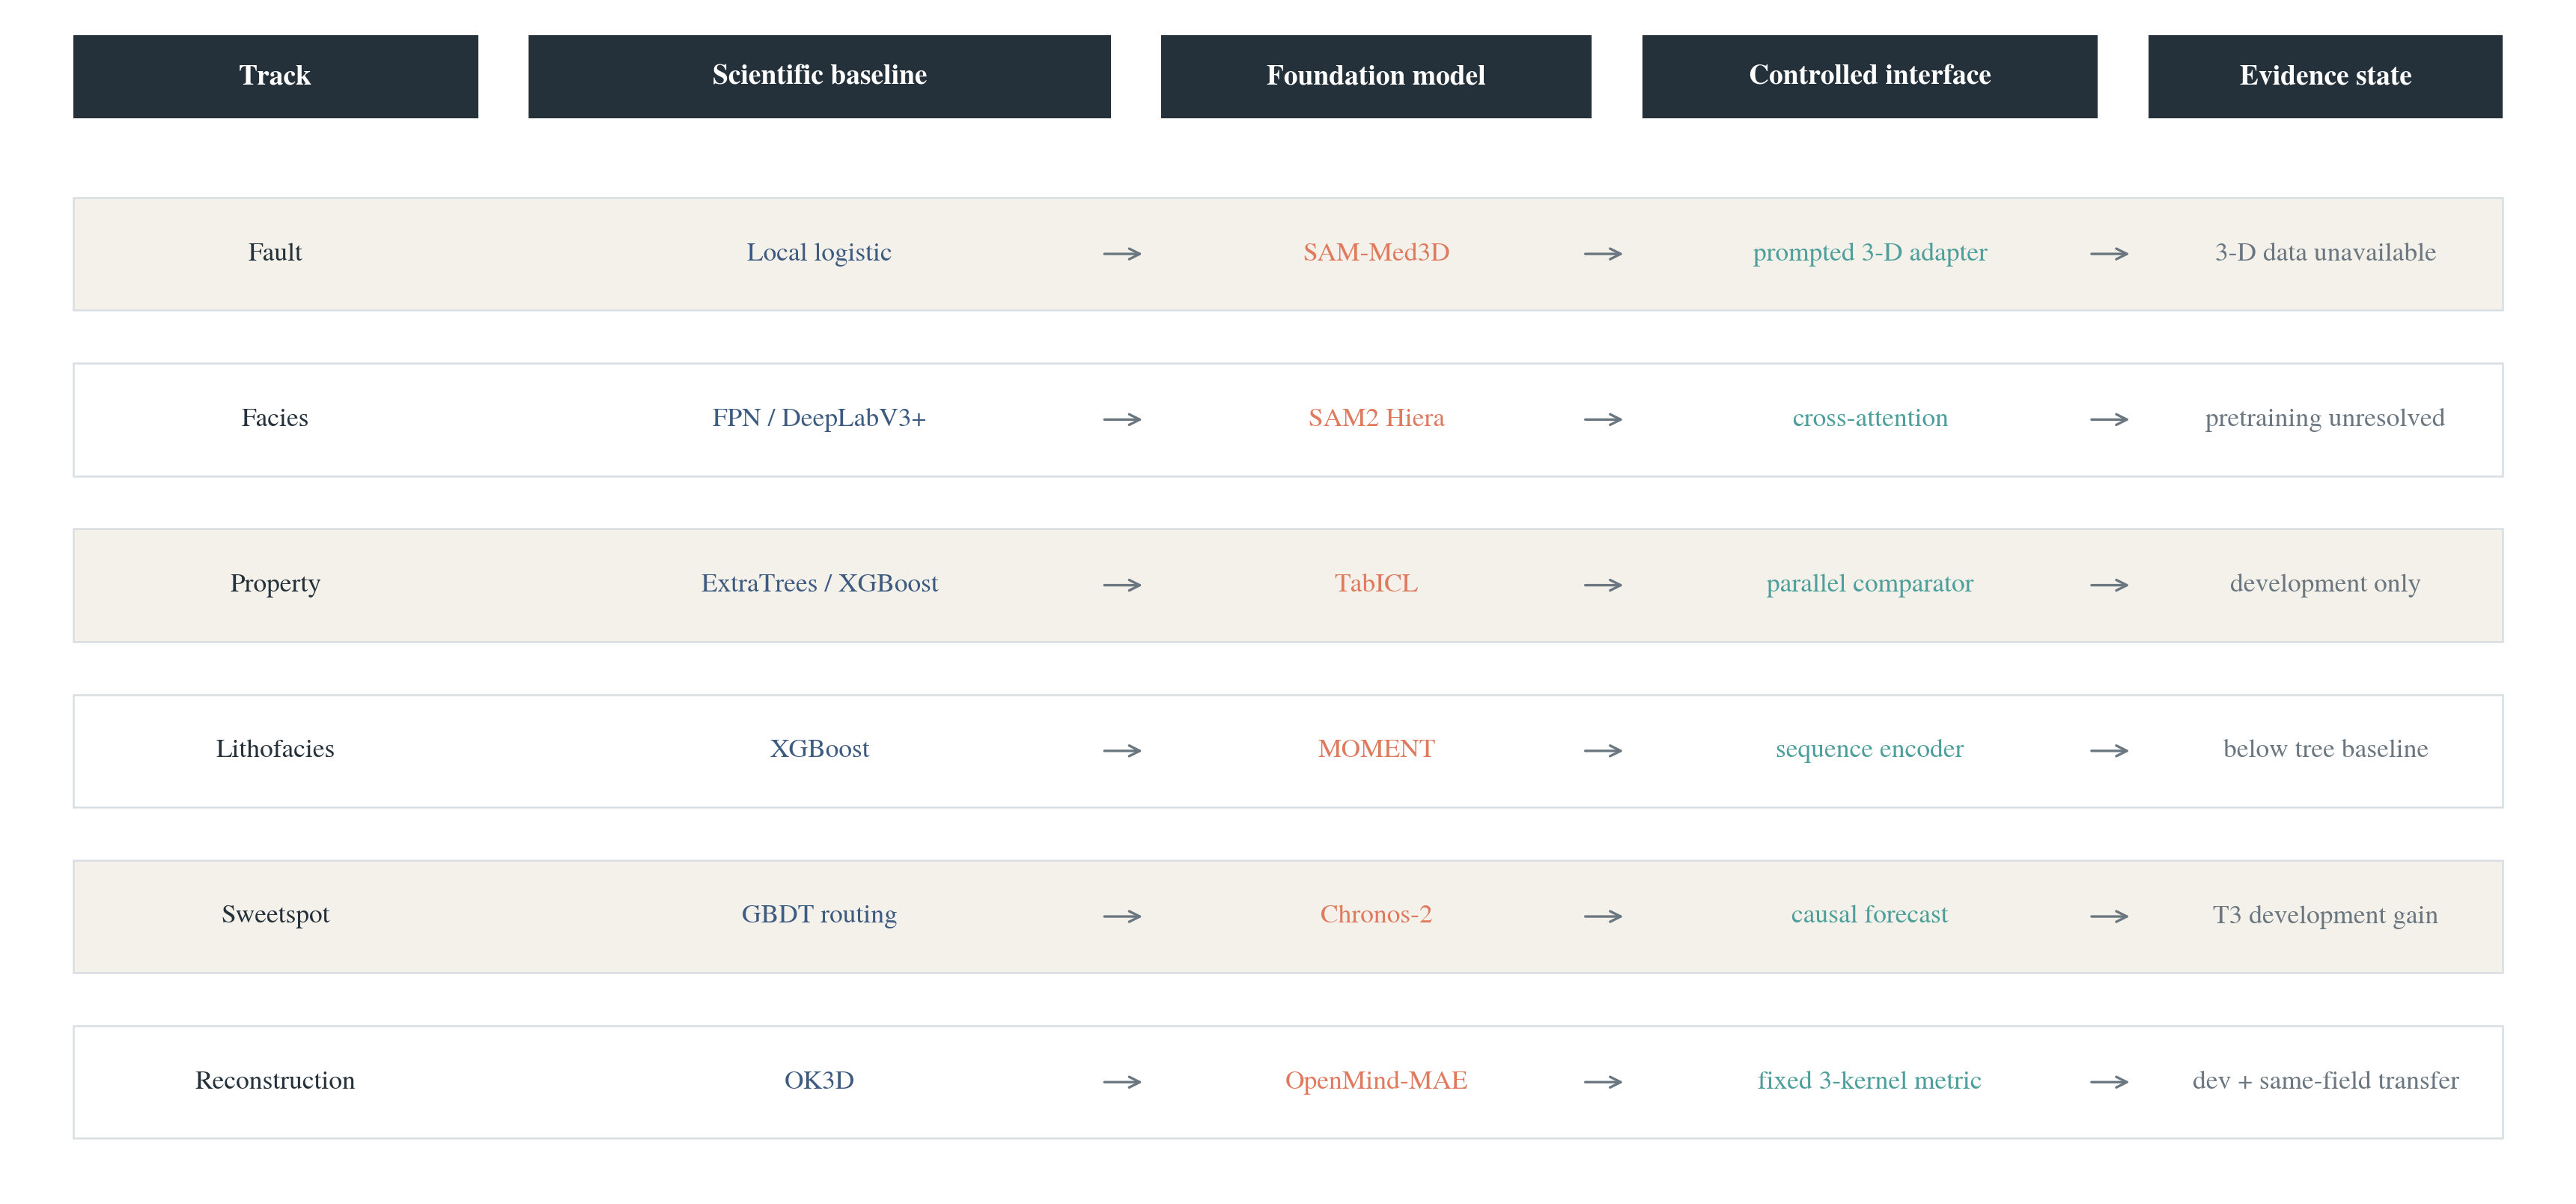
\includegraphics[width=0.98\textwidth]{../figures/results/foundation_model_research_map.png}
  \caption{六赛道基础模型研究设计。各赛道以强基线为参照，预训练模型分别通过独立
  对照、注意力融合、时序预测或邻域度量进入实验，并在固定划分下评价。}
  \label{fig:foundation-model-research-map}
\end{figure}

\section{实验原则}

所有赛道遵循三个原则。第一，数据划分先于模型训练确定，模型选择不得接触测试标签。
第二，主要评价指标在实验前固定，辅助指标只用于解释误差。第三，模型收益必须与
合理对照比较，包括强基线、历史均值、随机初始化或无基础模型分支。

对于已经被多次使用的留出集，本报告明确称为“已知留出集”，不把它包装成新的盲测。
对于没有合法开发折的任务，本报告只陈述基线结果，不推断候选模型已经胜出。这样的
表达可能更保守，但更接近实验事实。
